\documentclass{article}
\usepackage[margin=1in]{geometry}
\usepackage{graphicx}
\graphicspath{ {ConstructionPics/} }

\begin{document}
\title{\bf Applied Aeronautics \& OpenUAS: Albatross Construction Instructions and Notes}
\author{Madison Harrington}
\maketitle


\textbf{Contents}
\begin{enumerate}
\item Safety Considerations
\item Propellor
\item Servos
\item Lidar and GPS
\item Airspeed Sensor
\item Telemetry
\item Avionics 
\item Conclusions \newline
\end{enumerate}
The OpenUAS team followed the instruction provided by Applied Aeronautics for the majority of the construction of the Albatross UAV, but there were some minor adjustments to the procedure that are noted in detail in this document. All images were taken by OpenUAS team members.
Applied Aeronautics has a useful file for 3D prints, miscellaneous photos, and some instruction:

\ \

https://files.appliedaeronautics.com/Login \newline
Login: aacustomer \newline
Password: endurance \newline

\ \ 
\clearpage
\section{Safety Considerations}

It is recommended to wear a mask, safety goggles and keep the room in use ventilated while drilling into the Albatross. Spraying the surface with water before drilling is also recommended to mitigate the dust and cracks in the paint. \newline
\clearpage

\section{Propellor} 
Included in this section are steps in how our OpenUAS team assembled the propellor and images of the process. The propellor from the Applied Aeronautics kit did not fit on the screw assembly that they instructed to make. Therefore, the propellor's hole was increased to allow the assembly. The assembly was made to mimic the Applied Aeronautics' instructions, though some of the pieces did not match their kit so there was also some improvisation in the layers.

\begin{enumerate}

\item On the propellor, use a dremel to allow the screw to fit through propellor. Be careful to make an even and circular shape and to only increase the diameter as needed to fit on to the mount. Make small changes with the dremel and frequently check the fit to the mount's screw.
\item Layer all the pieces together as shown in the images below. The circular disk should be on bottom with the screw through that. Use the two washers on top of the large circular disk, then the propellor, and a nut on top of that. Ensure that everything is very secure. 
\item Choose the smallest screw from the kit (or the largest that fits to the bottom of the large screw). This will be placed through the nose cap along with a small nut and into the large screw to secure the nose cap to the rest of the pieces. Ensure this is tightened well.
\end{enumerate}


\begin{center}
\includegraphics[scale=0.5]{prop3} \newline
Here you can see the screw fitting into the circular disk. \newline
\includegraphics[scale=0.5]{prop5} \newline
Here you can see the internal assembly outlined in step 2 above. \newline
\includegraphics[scale=0.5]{prop1} \newline
\includegraphics[scale=0.5]{prop4} \newline
Note here the hole in the top of the screw, this is where the screw through the nose cap screws into. \newline
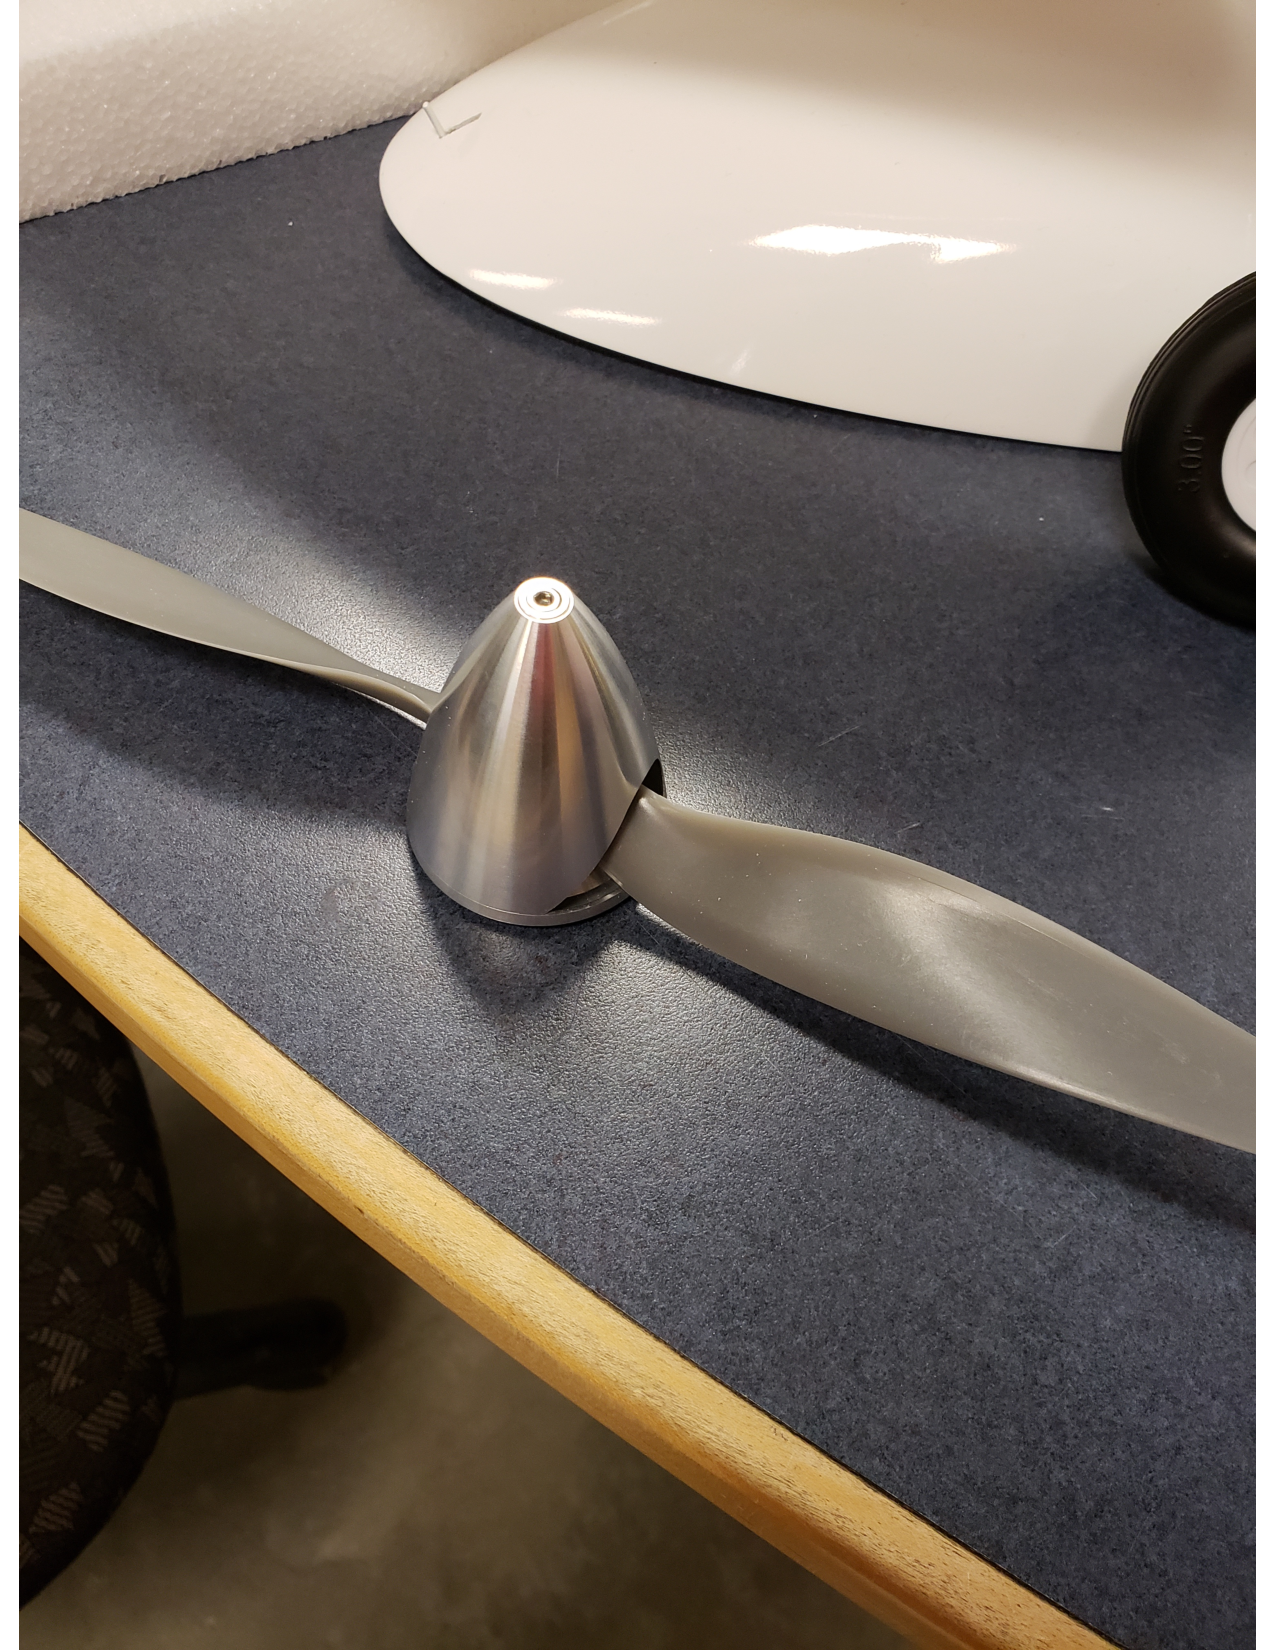
\includegraphics[scale=0.5]{prop2} \newline
Above you can see the final assembly, with the cap on the propellor and the screw through the top of the nose cap secured to the assembly. \newline

\includegraphics[scale=0.5]{motorinstal}
\end{center}

\clearpage
\section{Servos}

\subsection{Nose Wheel Servo}

\begin{center}
\includegraphics[scale=0.5]{nosewheelservo}
\end{center}


\clearpage
\subsection{Servo Holders}
   \begin {enumerate}
   \item Using the 3 3D print files for servo holders in the documentation. Print (with PLA filament):
   	\begin{itemize} 
	\item 3 HS-5085 holders
	\item 2 HS-5085 holders
	\item 2 HS-5245 holders 
	\end{itemize}
   \item Ensure that the servos snap nicely into the holders. 
   \item Use the softer side of the velcro sheets and stick these on the back of the servo holders. Use scissors and/or an exacto knife to cut these out.
   \end{enumerate}
   
\subsection{Servos}
   \begin{enumerate}
   \item *information regarding servo heads and screws*
   \end{enumerate}


\subsection{Servo connectors}
The servo connectors use 2 mm screws, a washer between the control surface and the first nut, then a nut underneath and on top of the joint link. There are three nuts total. (See the images at the end of this section)
\begin{enumerate}
\item Ensure that all the proper screws, washers and joint links are available as shown in the pictures. 
\item Using the $\frac{3}{32}$ inch drill, drill into the preset holes on each of the control surfaces (six in total).
\item Within the servo chamber, place one half of the velcro along the entire floor so that the servo can be positioned wherever desired. The back of the servo holders should have the opposite side of the velcro adhered to it. The servo can be screwed into the servo holder to minimize movement. 
\item Also be careful in how the servo is oriented when placed in the little groove. The white servo head should be free to move in the direction only away from the wing; so if it is sitting in the holder, the servo head should not move on the side of the holder. The head should also on the control-surface side of the servo chamber in order to make the joint-link connect to the control surface correctly.
\item Match the servo-joint link for matching control surfaces. The ailerons' joint links should be the same length so that inputs will actually match on both sides. This should be done for the flaps and rear controls as well.
\item Don't worry about which way the wires are facing in the servo chamber; the most important thing is to get the servo connected to the control surface, and secured. 
\item Once the servo is in place, use styrofoam or some sort of soft material to adhere to the inside of the servo cover (the white piece that screws over the servo hole). This is to compress the servo and mitigate any sort of movement against the velcro that it is sitting on. The cover should fit somewhat tightly once screwed in, just be careful not to add too much cushioning so that the screws are over stressed.
\item 
\end{enumerate}


\subsection{Aileron Servos}
You'll notice here construction completed as instructed by Applied Aeronautics: \newline

\begin{center}
\includegraphics[scale=0.5]{ServoConnection}
\end{center}

   
   Reference the following pictures.
   \newline
   
   \begin{center}
   \includegraphics[scale=0.5]{servoconnection1} \newline
   \includegraphics[scale=0.5]{servoconnection2} \newline
   \includegraphics[scale=0.5]{servoconnection3} \newline
   \includegraphics[scale=0.5]{servoholder1} \newline
   \includegraphics[scale=0.5]{servoholder2}\newline
   \end{center}
\clearpage

\section{Lidar and GPS}

\begin{enumerate}
\item Print the Lidar Stencil (from the Applied Aeronautics 3D print files) 
\item Unscrew and remove the rectangular carbon fiber tray from inside the fuselage. This should reveal the bottom of the fuselage for easy drilling. 
\item Place the 3D printed Lidar stencil in the fuselage approximately 3cm from the front edge of vertical carbon fiber brace.
\item Trace the outside of the stencil on the inside of the fuselage. Use a needle tool to poke through the fuselage in both holes with the given holes in the stencil. This represents the center of each lens. 
   \begin{itemize}
   \item NOTE: Be sure to pierce all the way through the skin of the fuselage.
   \end{itemize}
\item Flip the fuselage upside down (bottom facing up).
\item Align the stencil with the same holes just punctured and trace the outline of the lidar stencil. 
\item Using the two pin holes as a guide, drill two 19mm holes centered at these pin holes.
   \begin{itemize}
   \item NOTE: We recommend drilling smaller holes such as $\frac{5}{8}$ inches then using a dremel to fill in the stencil?s outline. This is to        be done with caution, doing fittings of the lidar in between dremeling.
   \end{itemize}
\end{enumerate}

\begin{center}
\includegraphics[scale=0.5]{LIDAR}
\end{center}

\clearpage

\section{Airspeed Sensor}

\begin{enumerate}
\item The airspeed sensor should stick out of the front of the Albatross like a Narwhal. Use a flashlight and note the white crease of the front of the inside of the nose.
\item Lay the airspeed sensor flat on the internal shelving and mark a hole at the point of the inside of the nose where you intend to drill.
\item Using your fingers, estimate where the hole will lead to the outside of the fuselage. 
   \begin{itemize}
   \item NOTE: There is no good way to drill the hole, so estimate as best as possible from the outside.
   \end{itemize}
\item Drill small hole where you marked, directly into the front of the nose of the Albatross (this hole should be above the point of the nose) parallel to the longitudinal axis of the fuselage. 
\item Compare this small hole to the mark on the inside of the fuselage and adjust as necessary. 
\item Slowly drill a 4mm hole parallel to the longitudinal axis of the fuselage. Check to see if the airspeed sensor fits in this hole. 
\end{enumerate}

\begin{center}
\includegraphics[scale=0.5]{airspeed}
\end{center}

\clearpage


\section{Telemetry}

\subsection{Drilling}
Holes will be needed on the panels that cover the telemetry on the Albatross. The recommended procedure for doing this is as follows:
\begin{enumerate}
\item Trace out the telemetry unit (the black grid and two antenna) so that the antenna fit in the storage area on the body part of the Albatross wing. There should be a hole so the square grid can face the open air for cooling purposes. The two antenna will also need holes through the panel so trace small circles where they align with the square drill site. Be careful to leave adequate room for wire connections since the tube that enters this region 
\item Use a dremmel with a fine tip to begin each of the drill sites. Be careful to stay within the trace lines drawn in the step above so that holes are not over-drilled. 
\end{enumerate}
\clearpage

\section{Avionics}
The following images show the wiring and organization of the main body of the Albatross UAV, before the addition of the battery. Note that hook and loop was used to secure the pixhawk and other components inside the fuselage. All the wiring is also tied off and organized for ease in making adjustments and testing individual components.\newline 

\begin{center}
\includegraphics[scale=0.1, angle=270]{Avionics1.jpg} \newline
\includegraphics[scale=0.1, angle=270]{Avionics2.jpg}


\end{center}

\subsection{Battery Care}
\subsection{Wiring and Soldering}
\subsection{Taranis}



\clearpage

\end{document}


